% !TEX root = ./article.tex

\documentclass{article}

\usepackage{mystyle}
\usepackage{myvars}



%-----------------------------

\begin{document}

	\maketitle % Insert title

	\thispagestyle{fancy} % All pages have headers and footers


%-----------------------------
%	ABSTRACT
%-----------------------------

	\begin{abstract}
		\noindent [TODO ]
	\end{abstract}

%-----------------------------
%	TEXT
%-----------------------------


	\section{Introducción}
	\label{sec:introducción}

		\paragraph{}
		[TODO]

		\subsection{Perceptrón Simple}
		\label{sec:simple_perceptron}

			\paragraph{}
			[TODO ]


		\subsection{Adaline}
		\label{sec:adaline}

			\paragraph{}
			[TODO ]

	\section{Perceptrón Simple sobre conjunto de datos sencillo}
	\label{sec:e1}

		\paragraph{}
		[TODO]

		\begin{table}[H]
			\centering
			\begin{tabu}{ | c | c | c |}
				\hline
				\multicolumn{3}{ | c | }{Simple Dataset} \\ \hline
				\bfseries $x_1$ & \bfseries $x_2$ & \bfseries $d(x)$
				\csvreader[head to column names]{../datasets/simple.csv}{
				  1=\one, 2=\two, 3=\three
				}
				{\\\hline\one&\two&\three}
				\\\hline
			\end{tabu}
			\caption{[TODO]}
			\label{table:e1_dataset}
		\end{table}


		\begin{figure}[h]
			\begin{center}
				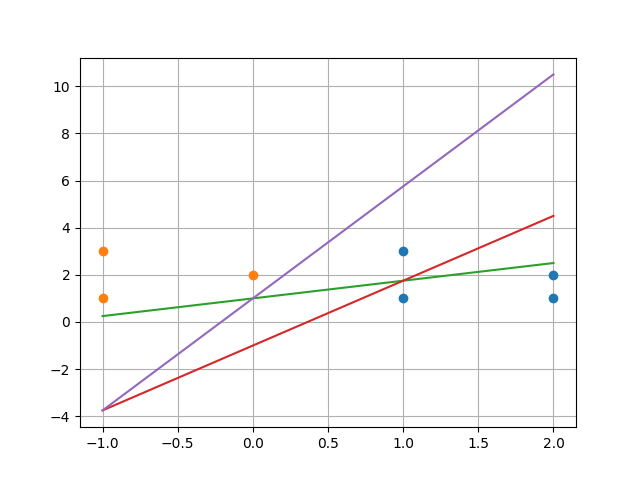
\includegraphics[width=0.75\textwidth]{simple-perceptron}
			\end{center}
			\caption{[TODO]}
			\label{fig:e1_plot}
		\end{figure}

		\begin{table}
			\centering
			\small
			\begin{tabu}{ | c | c | }
				\hline
				\multicolumn{2}{ | c | }{Perceptrón Simple - Simple Dataset} \\ \hline
				Error de Resubstitucion & $0.0\%$	 \\
				\hline
			\end{tabu}
			\caption{[]}
			\label{table:e1_error}
		\end{table}

	\section{Adaline sobre Machine Dataset}
	\label{sec:e2}

		\paragraph{}
		[TODO]

		\begin{table}
			\centering
			\small
			\begin{tabu}{ | c | c | }
				\hline
				\multicolumn{2}{ | c | }{Adaline --- Machine Dataset} \\ \hline
				Error HoldOut & $71.429\%$	 \\
				\hline
			\end{tabu}
			\caption{[TODO ]}
			\label{table:e2_error}
		\end{table}

%-----------------------------
%	Bibliographic references
%-----------------------------
	\nocite{subject:taa}
  \bibliographystyle{alpha}
  \bibliography{bib/misc}

\end{document}
